\documentclass{article}
\usepackage[preprint]{neurips_2022}
\usepackage{amsfonts}       % blackboard math symbols
\usepackage{amsmath}
\usepackage{booktabs}       % professional-quality tables
\usepackage{float}
\usepackage[T1]{fontenc}    % use 8-bit T1 fonts
\usepackage{graphicx}
\usepackage{hyperref}       % hyperlinks
\usepackage[utf8]{inputenc} % allow utf-8 input
\usepackage{microtype}      % microtypography
\usepackage{xcolor}         % colors
\title{Bilingual Offline Transcriptions: Midway Report}
\author{
  Yizhen Yu \\
  Carnegie Mellon University\\
  Pittsburgh, PA 15213 \\
  \texttt{yizheny@andrew.cmu.edu} \\\And
  Henry Wu \\
  Carnegie Mellon University \\
  Pittsburgh, PA 15213 \\
  \texttt{zhenyuW@andrew.cmu.edu}
}
\begin{document}
  \maketitle
  \section{Introduction and Problem Setup}
  \subsection{Advancements in DNNs for Automatic Speech Recognition}
  \textbf{Automatic speech recognition (ASR)}, the process of transforming human speech into readable text, has long been an area of popular research in machine learning. Traditional models for ASR are often based on a hidden Markov model (HMM) and Gaussian mixture model (GMM) architecture that learn explicit acoustic, lexicon, and language models; since then, end-to-end deep-learning proposals have advanced ASR without the need for these explicit models, although in some cases a language model is provided to achieve better results.

  A number of such end-to-end model architectures have been proposed, including RNN-\footnote{\cite{Chan}}, transformer-\footnote{\cite{Vaswani}}, and conformer-based\footnote{\cite{Gulati}} methods, and have steadily chipped away at word error rate (WER) as a metric of performance on ASR tasks. However, these methods have largely focused on training and running on a single language---usually English---while situations that include bilingual speech are largely overlooked. We intend to explore a selection of these architectures to investigate the ease and effectiveness with which we may introduce bilingual support.
  \subsection{Bilingual Speech and Code-Switching}
  A common phenomenon in conversations involving bilingual individuals is code-switching, in which a speaker changes languages within a single unit of speech\footnote{\url{https://en.wikipedia.org/wiki/Code-switching}}. This can happen at a number of different levels—among different sentences in a conversation, among words or phrases in a sentence, and even among parts of a single word.

  This project will focus on the first one---complete sentences in one of two languages in which a model is trained will be provided as input to the model to evaluate its effectiveness in distinguishing and transcribing them. (This task is different from that of \textit{speech translation}, in which the input is in one language and the output is in another.) This is a problem that is noticeably underserved not only in the literature---the only two papers we could find that addressed multilingual training are described in \ref{literature}---but also in implementation---even mature speech transcription services such as YouTube's automatic captioning service\footnote{\url{https://support.google.com/youtube/answer/6373554?hl=en}} fails to handle well-separated speech in two languages.
  \subsection{Data} \label{data}
  The goal of this project is to demonstrate, experiment with, and evaluate the introduction of bilingual speech into different ASR model architectures and to compare the performance between different model implementations as measured by WER. The trained models will take input in the form of audio clips of human speech, randomly allocated to either Lithuanian or Slovak, and output readable transcripts for comparison to validated transcripts for evaluation.

  The data used is Mozilla's Common Voice 11 dataset\footnote{\url{https://commonvoice.mozilla.org/en/datasets}}, a crowdsourced collection of over 24 thousand hours of audio clips in dozens of languages. (Some troubleshooting work is done with Common Voice 5, as described below, simply because it's more tightly integrated into the ESPnet software.) In particular, the Lithuanian and Slovakian datasets were selected for two reasons:
  \begin{itemize}
    \item They are relatively small but complete, with 15--20 hours of validated audio data each.
    \item They are both in the Latin script, limiting the output character space of the model.
  \end{itemize}
  In real-world terms, using this data simulates an ASR task on a conversation between people who speak Lithuanian and Slovakian.
  \subsection{Background and Literature} \label{literature}
  \cite{Yilmaz} investigates bilingual speech recognition between Dutch and Frisian, a minority language spoken in the North of Netherlands. As the two languages are influenced by each other, code-switching is common among speakers. The authors experiment on 3 sets of datasets using 2 different methods: language dependent training and independent training (see \ref{diagram yilmaz}). The former model is trained on each language separately by giving phones its specific language lexicon, while the latter includes mapping phones associated with the same IPA (International Phonetic Alphabet) symbol. They conclude that the latter language independent model achieves better accuracy and helps recognition of Frisian words. This is the most directly related prior art to our experiment.
  \begin{figure}[H]
    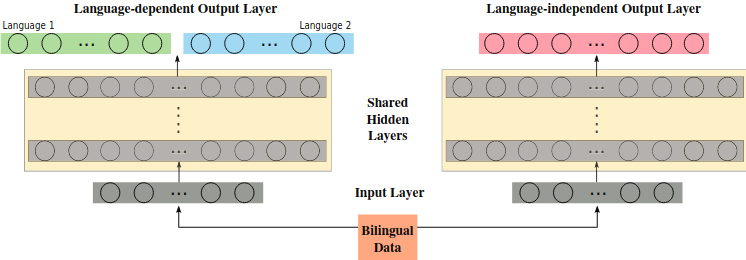
\includegraphics[width=\textwidth]{images/diagram-yilmaz}
    \caption{Language-dependent and language-independent architectures by \cite{Yilmaz}.}
    \label{diagram yilmaz}
  \end{figure}
  Note that as the authors point out, Dutch vowels are a subset of Frisian vowels and the two languages are strongly influenced by each other, which may make the combined model easier to train in that case. Although the two languages we intend to train on also use the same script, they are only very distantly related---Lithuanian is in the Baltic branch of the Indo-European language family, while Slovakian is in the Slavic branch. We would thus expect fewer of the advantages that \cite{Yilmaz} saw in combining models for two more similar languages.
  
  \cite{Liu} develops multilingual machine translation on a wider variety of languages using the mBART model, with a sequence-to-sequence auto-encoder trained on large monolingual corpora in many languages and a transformer decoder, comparing performance on models pretrained on different numbers of languages (see \ref{diagram liu}).
  \begin{figure}[H]
    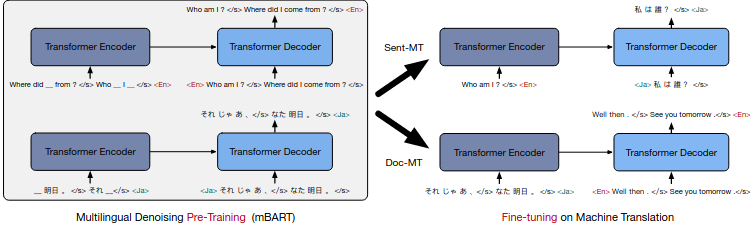
\includegraphics[width=\textwidth]{images/diagram-liu}
    \caption{Training process for mBART model by \cite{Liu}}
    \label{diagram liu}
  \end{figure}
  Note that although this paper deals with machine \emph{translation} rather than transcription, it's notable for the approach it takes for distinguishing languages, by labelling sentences with a language marker. THe paper concludes that pretraining with a dataset that includes both languages in and out of test data helps with performance, implying that the hidden layers of the transformer model learn generalized features across different languages which allow it to perform well against languages in testing it had never encountered during training.
  \section{Methods and Model}
  \subsection{Framework and Benchmarking}
  For our experimentation framework, we use ESPnet2\footnote{\url{https://github.com/espnet/espnet}}, a comprehensive speech processing toolkit that provides a large number of model recipes out of the box, many of which are based on and cross-reference specific papers. In addition, it comes with some useful data pipelines that can be fed into these recipes, including Common Voice 5.

  As a basic benchmark, we trained a preconfigured conformer model on the Common Voice 5 Assamese dataset and a transformer model on AN4\footnote{\url{https://github.com/cmusphinx/an4}}. These are relatively small datasets useful for configuration, with 20 and 40 minutes of speech data, respectively. Although these datasets are too small to be reasonably used for experimentation, they were valuable for providing intuition around the resource requirements for training on larger datasets.
  \begin{center}
    \begin{tabular}{llllrr}
      \toprule
      Dataset                 & Model       & Platform         & Training time & Test WER \\\midrule
      \texttt{commonvoice-as} & conformer   & Colab (GCP)      &        4003 s &  100.0\% \\ % TODO
      \texttt{commonvoice-as} & conformer   & Local (GTX 1070) &        3357 s &  100.0\% \\ % TODO
      \texttt{an4}            & transformer & Colab (GCP)      &         682 s &   28.6\% \\ % TODO
      \texttt{an4}            & transformer & Local (GTX 1070) &         948 s &   29.6\% \\\bottomrule
    \end{tabular}
  \end{center}
  \subsection{Preliminary Results}
  Our baseline model is to train ESPNet's conformer implementation from scratch on a randomly interleaved dataset containing sentences from both Common Voice 11 Lithuanian and Common Voice 11 Slovakian (see \ref{data}). This is tantamount to treating the two languages as if they were a single one; as discussed in \ref{literature}, this is a bit of an odd assumption. Nonetheless, the model learned quite well.
  \begin{figure}[H]
    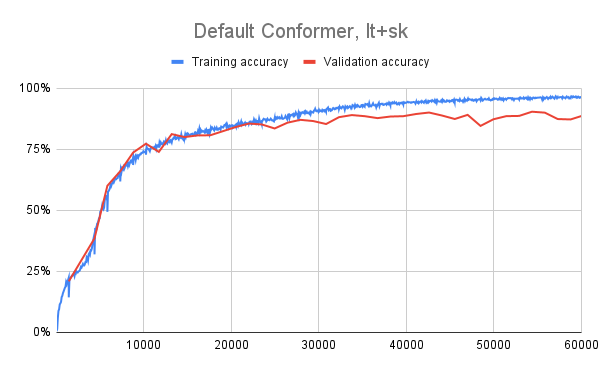
\includegraphics[width=\textwidth]{images/default-conformer_lt+sk}
    \caption{Training and validation accuracy from training a default ESPnet ASR conformer on a randomly interleaved dataset of Lithuanian and Slovakian samples.}
  \end{figure}
  \textit{[Author's note: It's taking a bit more time than expected to calculate the WER for the test data, which is why it was left out of the discussion above.]}
  \subsection{Evaluation of preliminary work}
  It was somewhat surprising how well the conformer handled the bilingual dataset out of the box, but it's possible to reason about it as the model learning a single language with a particularly deep orthography\footnote{\url{https://en.wikipedia.org/wiki/Orthographic_depth}}.
  \section{Future Work}
  \subsection{Approaches}
  In general, our experimental approach is to retrain our baseline conformer model with a few tweaks.
  \begin{enumerate}
    \item Inject an explicit language token (similar to \cite{Liu}) into the input data and see if it improves performance. \textit{[Will to complete by 30 Nov]}
    \item Train a language-dependent model (similar to \cite{Yilmaz}) with a shared encoder but separate decoders, and compare the WER resulting from the output from the "correct" decoder. \textit{[Henry to complete by 30 Nov]}
    \item As \cite{Liu} suggest in their paper on mBART experiments, machine translation performance is improved when training data include languages other than the ones present in test dataset. While our focus is speech recognition with bilingual transcripts, we can explore if adding audio input from other languages than our target (Lithuanian and Slovakian) improves performance. \textit{[assignee TBD]}
    \item \textit{[stretch goal, dependent on time]} Evaluate the performance of these experiments on transformer models (in addition to the default conformer). \textit{[assignee TBD]}
    \item \textit{[stretch goal, dependent on time]} As mentioned in mBART paper by \cite{Liu}, their model also has good performance even with unseen vocabularies in the testing set. We can also experiment to determine if an unseen language in the test dataset significantly decreases the accuracy of model trained on multiple languages.\textit{[assignee TBD]}
  \end{enumerate}
  \subsection{Further Investigation}
  Training the baseline model (default ESPnet conformer implementation) on the base Lithuanian and Slovakian datasets individually and evaluating their WERs on same-language test data would give us a more general baseline performance (that is, of an off-the-shelf monolingual ASR task) against which to compare our multilingual model.
  \newpage
  \bibliographystyle{plainnat}
  \bibliography{references}
\end{document}